
\begin{figure}[t]
  \centering
  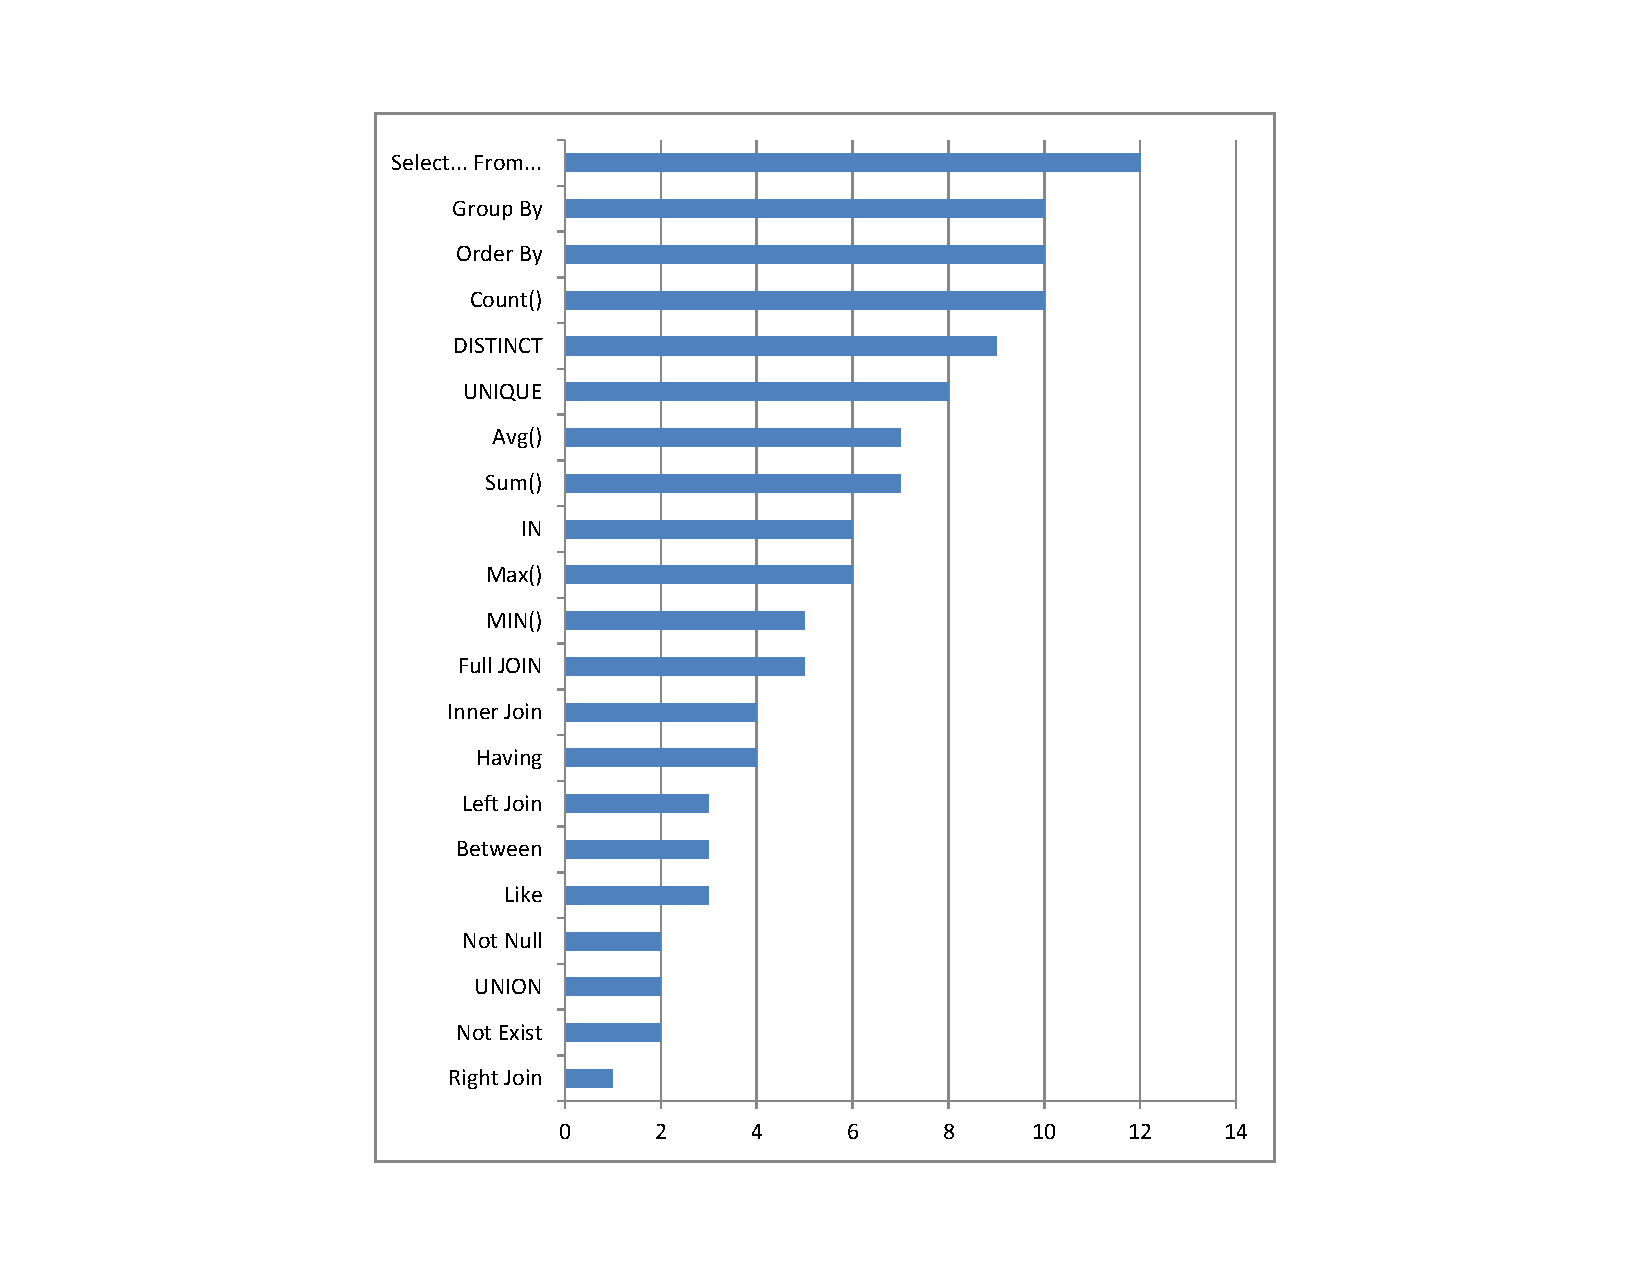
\includegraphics[scale=0.50]{survey}
  \vspace*{-1.0ex}\caption {{\label{fig:survey}
  \todo{remove distinct}
  Survey results of the most widely-used SQL features
  in writing a database query. There were 12 participants
  in the survey, and each participant was asked to
  select the top 10 widely-used SQL features.
  SQL features with no selection are omitted in this Figure
  for brevity.
}}

\end{figure}

\newcommand{\q}{\langle query\rangle}
\newcommand{\db}{\langle db\rangle}
\newcommand{\pat}{\langle pat\rangle}
\newcommand{\bug}{\langle bug\rangle}
\newcommand{\dist}{\langle distance\rangle}
\newcommand{\sem}[1]{\llbracket #1\rrbracket}
\newcommand{\lit}[1]{\texttt{#1}}

\newcommand{\column}{\langle column\rangle}
\newcommand{\dbtable}{\langle table\rangle}
\newcommand{\cond}{\langle cond\rangle}
\newcommand{\op}{\langle op\rangle}
\newcommand{\e}{\langle expr\rangle}
\newcommand{\ce}{\langle cexpr\rangle}

\begin{figure}[t]
%\scriptsize{%
\footnotesize%
\begin{align*}
\q ::= {} 
	& \texttt{ SELECT } \e^+ \texttt{ FROM } \dbtable^+ \\
        & \texttt{ WHERE } \cond^+ \\ 
	&  \texttt{ GROUP BY } \column^+ \texttt{ HAVING } \cond^+\\
	&  \texttt{ ORDER BY } \column^+ \\
\dbtable::= {} &\ atom \\
\column ::= {} &\ \dbtable.atom\\
\cond ::= {} &\ \ \cond \;\texttt{\&\&}\; \cond \\ 
    & |\ \cond \;\texttt{||}\; \cond \\
    & |\ \texttt{(}\;\cond\;\texttt{)} \\
    & |\ \ce \;\op\; \ce \\
\op ::= {} &\ \ \texttt{=} \;\;|\;\; \texttt{>}  \;\;|\;\; \texttt{<}\\
\ce ::= {} &\ \ const \;\;|\;\; \column  \;\; \\
\e ::= {} & \ce \;\;|\ count(\column) \\
    & |\ sum(\column) \;\;|\ max(\column) \;\;|\ min(\column) 
\end{align*}
\normalsize%
\caption{Syntax of the supported SQL subset in \ourtool.
%This subset covers the top XXX \todo{refer to figure 2}
%in Figure~\ref{fig:survey}
}
\label{fig:syntax}
\end{figure}


\section{A SQL Subset Supported in \ourtool}
\label{sec:langsubset}

Exact inference of queries for the whole
SQL language from examples
is infeasible in practice. As proved
by Sarma et al.~\cite{DasSarma:2010}, even for
a simplified SQL language, inferring
a SQL query satisifying a input-output example
pair is a PSPACE-Complete problem. To make our
technique usuable, we need to identify a
SQL subset using which a large class of query tasks
can be performed, and then design an efficient
algorithm to infer queries using that SQL subset.

Unfortunately, when designing the supported SQL
subset, we found that no systematic
study has ever been conducted to this end,
and little empirical evidence has ever been provided
on which SQL features are widely-used in practice.
Without such empirical knowledge, deciding which
SQL subset to support remains difficult.

%\todo{Existing work some existing work, that the author decided
%the language subset. We reduce the bias of selecting features}

To address this challenge and reduce our personal bias
in language design, we first conducted an online survey
to ask experienced IT professionals about the most widely-used
SQL features in writing database queries (Section~\ref{sec:survey}).
Then, based on the survey results, we designed
a SQL subset (Section~\ref{sec:syntax}).  
We also sent the designed SQL subset to the survey participants
and conducted a series of follow-up email interviews
to confirm whether our design would be sufficient in practice.




%Identify a domain of data on which a large class of users struggle to perform repetitive operations that they can clearly describe with examples





\subsection{Online Survey: Eliciting Design Requirements}
\label{sec:survey}


Our online survey consists of 6 questions that can be
divided into three parts. The first part includes
simple demographic questions about participants.
In the second part, participants were asked to select
the top 10 most widely-used SQL features in their minds.
Instead of directly asking participants about the SQL
features, which might be vague and difficult to respond,
we presented them a list of \textit{all} standard
SQL features in writing a query.
Additionally, participants were asked to report their 
own experience in writing SQL queries in the third part of the survey.

%Before distributing our survey, we conducted pilot
%interviews with three graduate students with XXX experience
%at University of Washington. We ran the survey with them and
%made notes of their comments. According to their feedback,
%we refined the survey questions and adjusted the wording to
%make sure that the questions are relevant and clear.


We sent out invitation to graduate mailing lists at
University of Washington, and posted our survey on
professional online forums (e.g., StackOverflow).
As of April 2013, we received \respnum responses.
On average, the respondents have 9.5 years of experience
in software development (max: 15, min: 5),
and 5.5 years of experience in
using database (max: 10, min: 2). In addition, two
participants identified themselves as database professionals.

Figure~\ref{fig:survey} summaries the survey results about
the most-widely used SQL features rated by 12 participants.

\subsection{Language Syntax}
\label{sec:syntax}

Based on the survey, we design a SQL subset
whose syntax is shown in Figure~\ref{fig:syntax}
%shown in
%that can contains
%many widely-used features required by real users. 
% shows the language syntax.


The supported SQL subset is a subset of the SQL 93
language. It covers all top 10 most widely-used SQL
features except for the \CodeIn{IN} keyword, plus
the \CodeIn{Having} keyword in Figure~\ref{fig:survey}. 
This SQL subset, though by means complete in writing all
possible queries, has significantly
enriched the SQL subset supported by many existing query inference
work~\cite{DasSarma:2010}. In particular, our SQL subset
supports writing queries across multiple tables,
conjuction of query conditions, aggregate functions
(i.e., \CodeIn{COUNT}, \CodeIn{MAX}, \CodeIn{MIN}, and \CodeIn{AVG}),
group by operations, and the \CodeIn{Having} clause.



When designing this SQL subset, we only considered standard
SQL features, and excluded
some vendor-specific features, such as the \CodeIn{top} keyword
which is supported in Microsoft SQLServer. 
We discard the \CodeIn{IN} keyword since it can be replaced
by a joining condition in most cases. For example:
\todo{}
We add the \CodeIn{Having} keyword because it is often used
together with the \CodeIn{Group by} clause.
For the unsupported features in Figure~\ref{fig:survey},
keywords \CodeIn{Full Join}, \CodeIn{Left Join}, and \CodeIn{Right Join}
provide special ways to join two tables, and are less
likely to be used by non-expert users in practice.
Keyword \CodeIn{Not Null} can be replaced
by a condition to check whether the decorated
column has a \CodeIn{Null} value or not.
Keyword \CodeIn{Between} can be replaced by two
conditions that check the value boundary. For example,
\todo{xxx.}. Keywords \CodeIn{UNION} and \CodeIn{Not Exist}
are often used in writing nested queries, which are
not currently supported in \ourtool.
Keyword \CodeIn{Like} is also not supported, since
\todo{string matching}




\subsection{Follow-up Interviews: Feedback about the SQL Subset}
\label{sec:interview}

After proposing the SQL subset in Figure~\ref{fig:syntax},
we performed follow-up email interviews to gain
participants' feedback about the tailored SQL
subset. Participants were first asked to rate
the expressiveness of the SQL subset in Figure~\ref{fig:syntax}
on a 6-point scale (5-completely
sufficient; 0-not sufficient at all;
and in-between values indicating intermediate sufficiency),
and then to provide their comments.

On average, the rating of this SQL subset is 4.5. Most of
the participant rate it 5, or 4. Only one participant rates
it 3, since he mistakenly thought this subset does not
support joining multiple tables. 

One participant commented that the SQL subset did not support
column re-naming. However, re-naming database columns is not
critical in sythesizing a correct SQL query \todo{xxx}

Overall, based on the feedback, we think our SQL subset is
sufficient for writing a wide range of database queries
that most end-users would need.

